\documentclass[11pt]{article}
\usepackage[a4paper,margin=22mm,headheight=16pt]{geometry}
\usepackage{fontspec,xeCJK,xcolor,graphicx,enumitem,fancyhdr,titlesec}
\usepackage{hyperref}
\IfFontExistsTF{Times New Roman}{\setmainfont{Times New Roman}}{\setmainfont{TeX Gyre Termes}}
\IfFontExistsTF{FangSong}{\setCJKmainfont[AutoFakeBold=2]{FangSong}}{\IfFontExistsTF{仿宋}{\setCJKmainfont[AutoFakeBold=2]{仿宋}}{\IfFontExistsTF{FandolFang-Regular.otf}{\setCJKmainfont[AutoFakeBold=2]{FandolFang-Regular.otf}}{\setCJKmainfont{FandolSong-Regular.otf}}}}
\definecolor{ink}{HTML}{173747}\definecolor{accent}{HTML}{227E82}
\hypersetup{colorlinks=true,urlcolor=accent,linkcolor=accent}
\linespread{1.22}\setlength{\parindent}{0pt}\setlength{\parskip}{6pt}
\setlist[itemize]{leftmargin=1.4em,itemsep=3pt}
\titleformat{\section}{\large\bfseries\color{ink}}{}{0pt}{}
\titlespacing*{\section}{0pt}{14pt}{7pt}
\pagestyle{fancy}\fancyhf{}\lhead{\small LEARNPATH / 学习手册}\rhead{\small Source-grounded learning}\cfoot{\small\thepage}
\emergencystretch=2em\widowpenalty=10000\clubpenalty=10000
\newcommand{\Needspace}[1]{\par\ifdim\dimexpr\pagegoal-\pagetotal\relax<#1\relax\newpage\fi}
\begin{document}


{\LARGE\bfseries\color{ink} 音乐通识：30天学习计划}\par

2026-10-08 | 学习计划 / 30 天\par\vspace{6pt}

\Needspace{5\baselineskip}\section*{学习者与目标}

适合：爱听音乐但不熟悉乐理的成年人。

本轮目标：用具体听觉线索描述作品，建立持续欣赏方法。30天用于建立入门框架与方法，不承诺掌握整个学科。除明确说明的基础外，不假设学习者的行业经历。原始启动句：“我想学习音乐，提升欣赏不同作品的能力。”

\Needspace{5\baselineskip}\section*{学习方式与时间安排}

每天预计10–15分钟：正文与读图约8分钟，回忆和练习约3分钟，可用余下时间复述。学习速度存在差异，时间为估计值；扩展阅读不计入必做量。每天10:00（Asia/Shanghai，含周末）开始生成，检查完成后交付。计划确认后可立即生成Day01。

本文件是公开演示样例：30天完整课纲，配套展示Day01–Day03；试跑不创建真实定时任务。图中A、B、C分别对应前三天的观察重点。

\begin{center}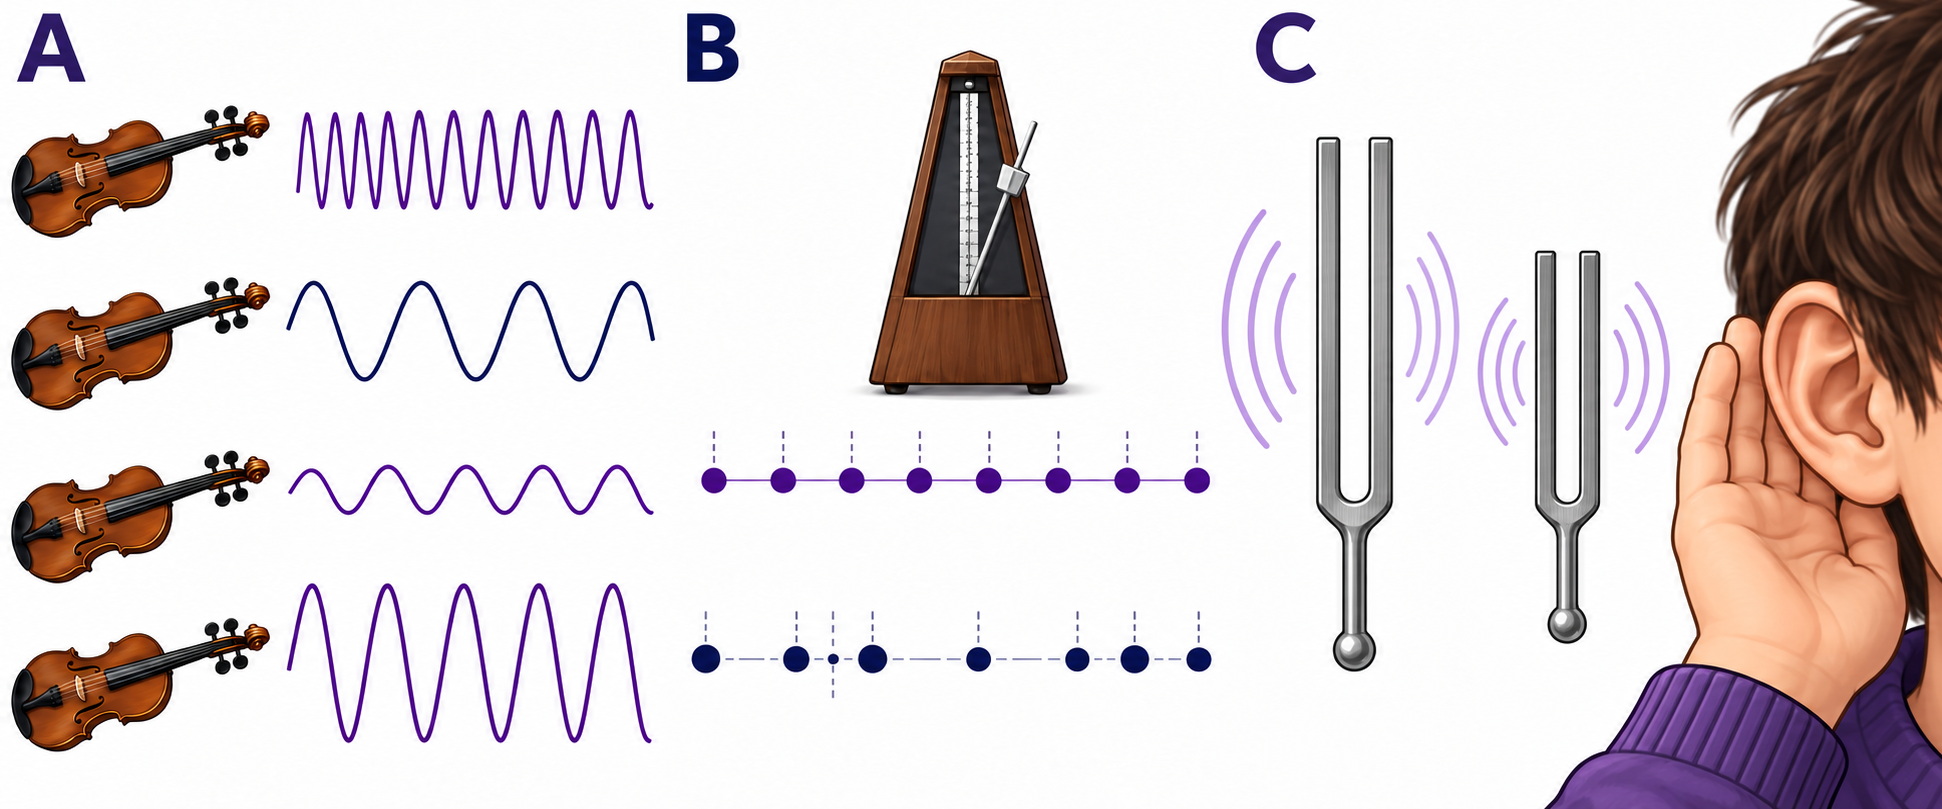
\includegraphics[width=\linewidth,height=0.26\textheight,keepaspectratio]{../assets/figure-f6141a0bb6d5.png}\par

{\small A 比较振动疏密与振幅；B 稳定脉冲和节奏事件并不相同；C 两个音高之间可以比较方向与距离。波形仅作概念示意。}\par

{\footnotesize AI生成教学示意，非实物照片、原始史料或官方架构。生成方式：内置文生图；提示词见仓库 docs/image-prompts.json。}\end{center}

\Needspace{5\baselineskip}\section*{课程依据与学习成果}

先从听见音高力度与音色进入，逐渐引入领域概念，再通过案例与复盘连接。来源[S1]和[S2]提供起点知识；其他链接扩展相关视角。课程排序是本项目的教学设计，不是来源机构为本项目背书。

完成时应能：分别描述高低强弱和音色；说明配器如何改变听感；设计可持续的聆听路径。每五天安排一次回顾或整合，检查能否脱离正文解释，不以“收到PDF”代替学会。

\Needspace{5\baselineskip}\section*{阶段1：主动聆听}

Day01  听见音高力度与音色
目标：分别描述高低强弱和音色。

Day02  节拍节奏与速度
目标：保持脉冲并辨认节奏事件。

Day03  旋律走向与音程
目标：画出乐句音高轮廓。

Day04  乐句与呼吸
目标：标记一句旋律的停顿。

Day05  复盘一次主动聆听
目标：提交三条可听见的观察。

\Needspace{5\baselineskip}\section*{阶段2：声音组织}

Day06  音阶与调性
目标：辨认稳定感与音阶关系。

Day07  和弦与伴奏
目标：听出伴奏与旋律的分工。

Day08  织体与声部
目标：比较单线和多线组织。

Day09  重复对比与曲式
目标：标出重复与变化。

Day10  复盘作品结构
目标：画一幅简单结构图。

\Needspace{5\baselineskip}\section*{阶段3：人声与乐器}

Day11  人声与合唱
目标：比较独唱与合唱的表达。

Day12  弦乐器的声音
目标：描述弓弦与拨弦差异。

Day13  木管与铜管
目标：寻找两种管乐音色线索。

Day14  打击与电子声音
目标：辨认打击和电子音色角色。

Day15  复盘配器选择
目标：说明配器如何改变听感。

\Needspace{5\baselineskip}\section*{阶段4：西方风格入口}

Day16  巴洛克音乐入口
目标：找出模仿或持续低音线索。

Day17  古典主义的对话
目标：描述乐句间的呼应。

Day18  浪漫主义的表达
目标：以具体声音支持情绪描述。

Day19  二十世纪的探索
目标：比较两种组织声音的方法。

Day20  复盘风格比较
目标：给两段作品写比较句。

\Needspace{5\baselineskip}\section*{阶段5：多元音乐经验}

Day21  中国音乐的线索
目标：承认不同传统的分析边界。

Day22  爵士与即兴
目标：辨认即兴与固定框架的关系。

Day23  流行歌曲的结构
目标：识别主歌副歌等功能段。

Day24  影视音乐与情境
目标：说明情境如何改变感受。

Day25  复盘多元聆听
目标：比较同一方法的适用范围。

\Needspace{5\baselineskip}\section*{阶段6：比较与表达}

Day26  演奏版本的差别
目标：记录两版演奏的具体差异。

Day27  录音与现场
目标：比较空间与制作影响。

Day28  如何查作品资料
目标：找到可靠作品版本信息。

Day29  写一段有证据的乐评
目标：用观察支持一段评价。

Day30  结业：个人聆听地图
目标：设计可持续的聆听路径。

\Needspace{5\baselineskip}\section*{自测、调整与确认}

每天先尝试作答，再看参考要点；答不出来时记录具体概念，不据此给自己贴能力标签。每五天用一张卡整理“已经能解释／仍不确定／需要查证”。若学习量过大，优先缩小每日范围并保留主线，不靠减小字体压缩材料。

真实使用时，请确认目标、基础、周期、每天用时、执行时间、时区与输出目录。批准当前计划后才创建任务；修改已开始的课程时保留旧档案并建立新版本。到期漏跑则继续最早未交付课程，不按日期跳课。

\Needspace{6\baselineskip}\section*{扩展学习 / Further reading}\small 以下为选读，不计入每日必做时间。\begin{enumerate}[leftmargin=1.6em]

\item [S1] \href{https://openstax.org/books/physics/pages/14-1-speed-of-sound-frequency-and-wavelength}{Speed of Sound, Frequency, and Wavelength} — 选读声音频率与音高的关系，公式推导可跳过。\par OpenStax | 发布：未标注 | 核验：2026-10-08

\item [S2] \href{https://openmusictheory.github.io/basicNotation.html}{Basic notation} — 认识音符、谱表和变音记号；本课不要求记住全部符号。\par Open Music Theory | 发布：未标注 | 核验：2026-10-08

\item [S3] \href{https://openmusictheory.github.io/rhythmicValues.html}{Rhythmic values} — 观察长短时值和休止符如何表达时间。\par Open Music Theory | 发布：未标注 | 核验：2026-10-08

\item [S4] \href{https://openmusictheory.github.io/meter.html}{Meter and time signatures} — 选看拍子分组与聆听示例；部分嵌入播放器可能需要额外登录。\par Open Music Theory | 发布：未标注 | 核验：2026-10-08

\item [S5] \href{https://openmusictheory.github.io/intervals.html}{Intervals and dyads} — 重点看半音数与音程度数不是同一种计数方法。\par Open Music Theory | 发布：未标注 | 核验：2026-10-08

\end{enumerate}

\end{document}